\chapter*{Resumen ejecutivo}
\section*{Introducción}
Los cuadricópteros son vehículos aéreos no tripulados (\textit{UAV}) que se emplean para una gran variedad de tareas, por ejemplo, para la inspección de las palas de un aerogenerador en movimiento, el rodaje de una escena de acción en medio del mar o para facilitar la búsqueda de personas a las fuerzas del estado en labores de búsqueda y rescate. Estas aeronaves son iherentemente inestables, por lo que es necesario que cuenten con un sistema, que se encargue de mantener a la aeronave estable y facilitar su pilotaje. El desarrollo de los algoritmos de control que se ejecutan en estos sistemas, es un campo de interés debido a la utilización masiva de estas aeronaves, en tareas de naturaleza muy diversa.

\section*{Alcance}

Los objetivos de este trabajo son: diseñar una plataforma real segura, en la que se pueda probar y evaluar el rendimiento de distintos algoritmos de control de cuadricópteros y diseñar y probar algoritmos de control novedosos empleando las últimas técnicas de aprendizaje por refuerzo y aprendizaje profundo. Esta plataforma puede ser usada tanto para la labor investigadora (a la hora de desarrollar nuevos algoritmos de forma segura), como para la labor docente (enseñar las técnicas de control clásicas en una plataforma real).

Para acometer este proceso, se ha desarrollado un autopiloto en el que poder ejecutar los algoritmos de control que se diseñen, a bordo de la aeronave y un cuadricóptero en el que realizar los experimentos.

Adicionalmente, se ha empleado un entorno de simulación en el que se han desarrollado y validado los distintos algoritmos de aprendizaje por refuerzo que se han propuesto.

\section*{Solución realizada}

\begin{itemize}
	\item \textbf{Diseño del autopiloto}. Un autopiloto es el sistema encargado de estabilizar y comandar a la aeronave a bajo nivel. Con el objetivo de poder implementar los algoritmos de control sin restricciones, se ha diseñado un autopiloto propio con toda la electrónica necesaria para poder controlar un cuadricóptero \cref{hardware:carl_board}.  

\begin{figure}[htb!]
	\centering
	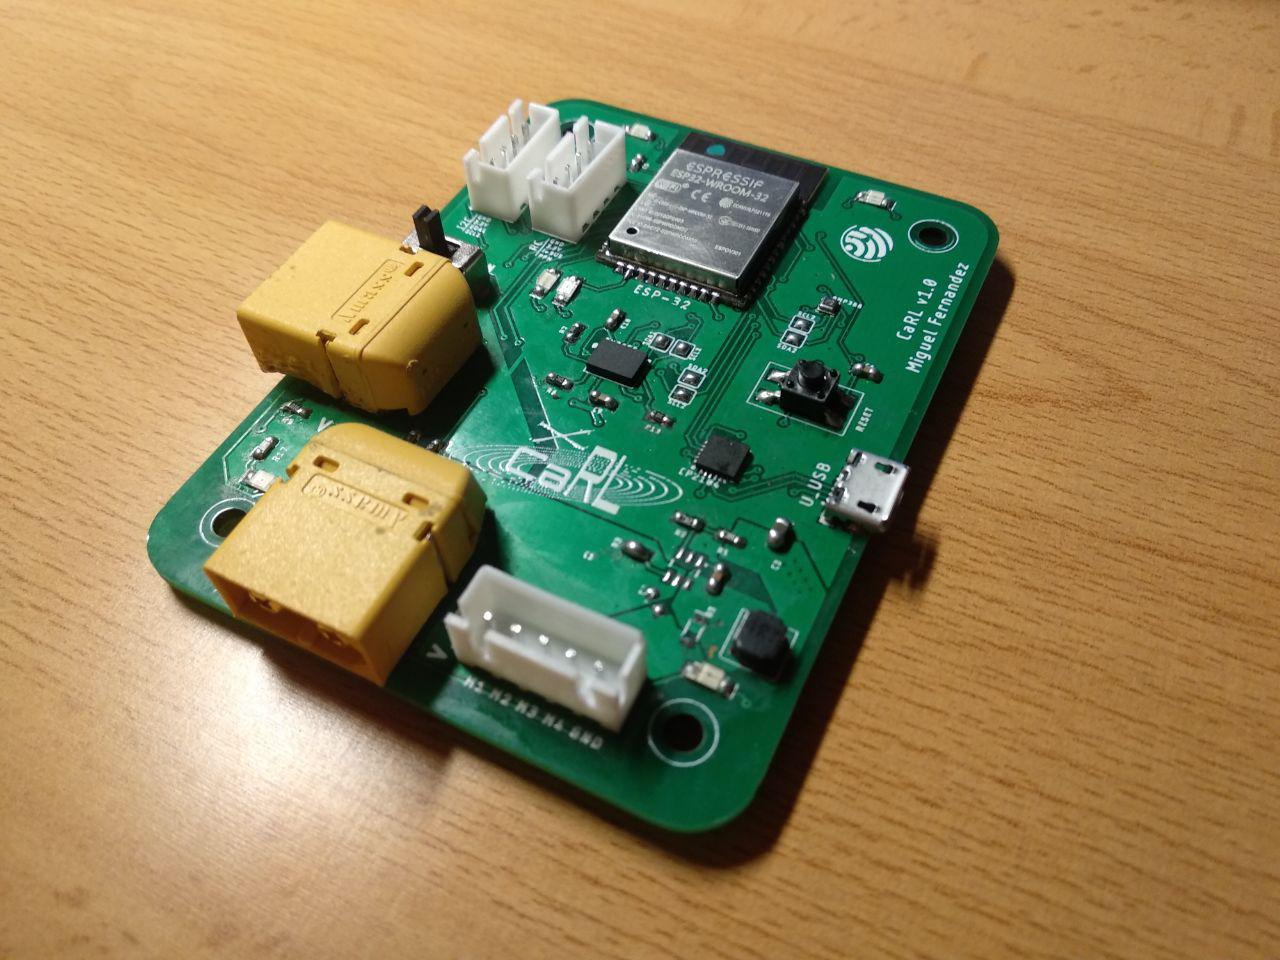
\includegraphics[width=0.\textwidth]{hardware/carl_board}
	\caption{Autopiloto CaRL (\textit{Cuadcopter with autopilot based on Reinforcement Learning}).}
	\label{hardware:carl_board}	
\end{figure}
	
	\item \textbf{Diseño del cuadricótpero y el banco de pruebas}. Para poder evaluar el rendimiento de los algoritmos de control empleados, es necesario contar con una plataforma real, en la que sea seguro probar estos algoritmos. Es por esto que se ha diseñado y construido un cuadricóptero, en el que montar el autopiloto y un banco de pruebas con diversas configuraciones, dependiendo del experimento que se quiera realizar.\tb{imagen}
	
	
	\item \textbf{Desarrollo de algoritmos de control basados en aprendizaje por refuerzo}. Con el ánimo de encontrar métodos de control novedosos, que sean capaces de controlar a los cuadricópteros de forma más eficaz, se ha experimentado con los distintos algoritmos de estado del arte en el campo del aprendizaje por refuerzo.
	
\end{itemize}


\section*{Experimentación y resultados.}
Se han realizado experimentos tanto en la plataforma real como en simulación.

En la plataforma real se ha probado el funcionamiento del autopiloto, la aeronave y el banco de pruebas empleando algoritmos de control clásico, con los que se ha conseguido estabilizar la plataforma en diferentes configuraciones.

En el entorno simulado, se ha comparado el rendimiento de los algoritmos de control empleando aprendizaje por refuerzo, con el algoritmo de control clásico PID (Propocional-Integral-Derivativo). En estos experimentos se ha observado como alguno de los algoritmos empleados, como el TRPO, son capaces de conseguir respuestas con características dinámicas muy satisfactorias. 

\section*{Conclusiones y trabajo futuro}
Se ha conseguido desarrollar una plataforma que permite probar de forma segura distintos algoritmos de control en cuadricópteros, esta plataforma se podría redimensionar para poder ser empleada en institutos y universidades con el ánimo de facilitar el aprendizaje de la teoría de control mediante la interacción directa con un sistema tan atractivo, como el de un cuadricóptero.

Desde el punto de vista del algoritmo de control, se ha conseguido entrenar agentes capaces de estabilizar un cuadricóptero en simulación con resultados prometedores, eso abre el paso a intentar mejorar estos algoritmos con el propósito de conseguir controladores mas precisos y eficaces.

\section*{Palabras clave}
UAV, cuadricóptero, control clásico, aprendizaje automático, inteligencia artificial, aprendizaje por refuerzo, redes neuronales.
\section*{Códigos UNESCO}
\begin{itemize}
	\item[] $120304$ \quad INTELIGENCIA ARTIFICIAL
	\item[] $120326$ \quad SIMULACIÓN
	\item[] $330104$ \quad AERONAVES
	\item[] $330412$ \quad DISPOSITIVOS DE CONTROL
	\item[] $330703$ \quad DISEÑO DE CIRCUITOS 


\end{itemize}
\newpage
\newpage